\subsubsection{Gestão de fases e entregas}
\label{ssub:gestao_fases}

Na página dedicada à gestão de fases e entregas, um docente pode consultar e editar todas as informações das fases de um projeto e todas as entregas relativas às referidas fases.

Relativamente às fases, num plano principal, são apresentadas informações relativas às datas de inicio e de fim da fase, descrição, ficheiros de entrega obrigatória, ficheiros auxiliares, e atalhos para a pauta e para o enunciado da fase. Para cada fase, um docente pode consultar estatísticas, publicar a pauta e verificar quais os grupos que já efetuaram entregas válidas.

Ao carregar numa entrega é possível avaliar individualmente cada aluno. Para cada aluno, um docente pode deixar um comentário sobre a nota atribuída. Para auxiliar na da nota dada, o docente pode consultar resultados dos testes efetuados.

Na Figura~\ref{fig:teacher_deliveries} pode ser consultada uma imagem demonstrativa da página desenvolvida.

\begin{figure}[H]
  \centering
  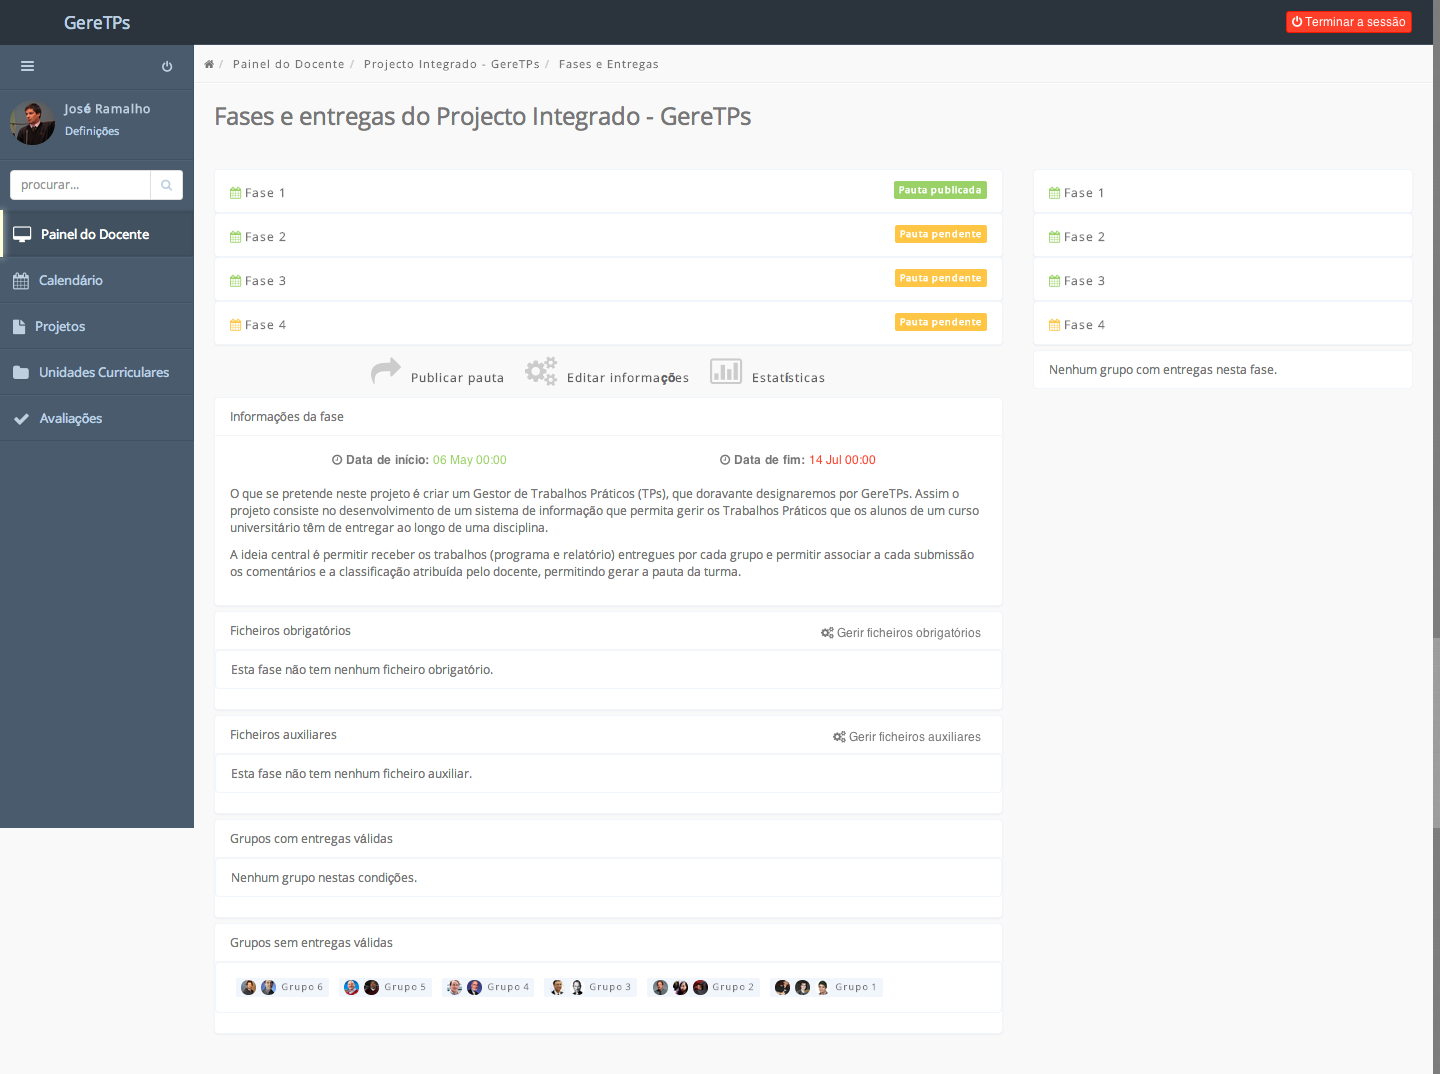
\includegraphics[width=1\textwidth,center]{images/implementacao/docentes/deliveries}
  \caption{Página de gestão de fases entregas}
  \label{fig:teacher_deliveries}
\end{figure}
